% Statt "de" kann hier auch "en" stehen, wenn die Arbeit auf Englisch verfasst wird
% Entweder "darkstyle" oder "lightstyle"

\documentclass[de, darkstyle]{unirostock}
\usepackage{float}
\usepackage[bottom]{footmisc}
\usepackage{minted}
\usepackage{listings}
\usepackage{colortbl}
% Für die Quellenangaben, weitere Informationen https://de.overleaf.com/learn/latex/Bibliography_management_with_biblatex
\usepackage[backend=biber,style=alphabetic,maxbibnames=99,backref=true,citestyle=alphabetic]{biblatex}
\addbibresource{lit.bib}
\DeclareFieldFormat{titlecase}{#1} % Optional: Titelstil setzen
\defbibheading{bibliography}[]{%
  \chapter*{\color{uniblau}\huge\sffamily\normalfont \textit{Literatur}}%
}
% Welche Bedingungen gibt es für die Verbreitung der Arbeit?
% creative-commons: Creative Commons Lizenz, Namensnennung - Weitergabe erlaubt unter gleichen Bedingungen 
% private: Veröffentlichung und Veränderung nur nach Rücksprache mit dem Autor
\license{creative-commons}

\author{Jakob Engelbert Tomahogh}
\enrolmentnumber{221201101} % Matrikelnummer

\title{Sicherheitsanalyse durch Entwicklung eines Rogue Device zur Echtzeitmanipulation maritimer Steuerungssysteme}
\type{Bachelorarbeit}

\course{Informatik}
\workperiod{15. November 2024 -- 04. April 2025}
\primaryreviewer{M. Sc. Marvin Davieds}
\secondaryreviewer{Prof. Dr. rer. nat. Clemens H. Cap} % Falls es keinen gibt, einfach weglassen

\faculty{Fakultät für Informatik und Elektrotechnik}
\institute{Institut für Informatik}
\workinggroup{Lehrstuhl für Informations- und Kommunikationsdienste}

\begin{document}
\maketitle
\makelicense

\pagenumbering{Roman}

\tableofcontents % Inhaltsverzeichnis.
\clearpage

\setstretch{1.263}
\pagenumbering{gobble}
\clearpage
{\normalfont
\color{uniblau}
\huge\sffamily\itshape
Abstract
}

In dieser Machbarkeitsstudie wird untersucht, ob die Steuerung eines Schiffes durch Manipulation von Steuergeräten möglich ist.
Es wird ein Rogue Device entwickelt, das externe Steurungsbefehle erhält und manipulierte Nachrichten auf die Schiffskommunikation sendet.
Dabei liegt der Fokus der Arbeit auf der Motorsteuerung über einen CAN-Bus. Die Rudersteuerung mit einer seriellen Schnittstelle wird kurz betrachtet.
Eine zentrale Fragestellung ist dabei, wie die Manipulation von Steuergeräten erschwert werden kann.
Durch die Simulation eines Angriffs wird gezeigt, dass die Steuerung eines Schiffes durch Manipulation von Steuergeräten möglich ist.
Jedoch wird zusätzliche Forschung benötigt, um eine tatsächliche externe Steuerung zu ermöglichen.
Dadurch werden verschiedene Sicherheitslücken an dem CAN-Bus und dem J1939-Standard aufgezeigt.
Die Ergebnisse dieser Arbeit sind auch für andere Schiffe relevant, da der CAN-Bus weit verbreitet ist.

\vfill
\clearpage

\pagenumbering{arabic} % Ab hier folgt die "arabische" Seitennummerierung.

% Im Ordner chapter sollte für jedes Kapitel eine Datei angelegt und hier eingebunden werden.
% Das erhöht die Übersicht.
% Description: Einleitung der Arbeit
\chapter{Einleitung}
\printmyminitoc{1}

\section{Motivation}
In der Seefahrt ist die Anzahl an Cyberangriffen in den letzten Jahren stark angestiegen. Von 2021 auf 2022 hat sich die Anzahl von öffentlich
bekannten Angriffen mehr als verdoppelt. Im Jahr 2021 sind lediglich 24 Angriffe bekannt geworden, im Jahr 2022 waren es bereits 65 Angriffe 
\cite{mcad}. Darunter fallen Angriffe auf Häfen, Schifffahrtsunternehmen und Schiffe.
Jedes Jahr werden zahlreiche Passagiere mit Schiffen befördert. Dabei kann es vorkommen, dass bösartige Aktoren ein Teil dieser Passagiere sind.
Ein Angriff auf die Steuerung eines Schiffes kann katastrophale Folgen haben. Dennoch ist die Sicherheit von Schiffen nicht 
immer ausreichend gewährleistet \cite{Reilly2016}.
Um das zu verdeutlichen, soll in dieser Arbeit durch physischen Zugriff auf ein Schiff die Kommunikation manipuliert werden.
Damit soll die Kontrolle über die Steuerung des Schiffes übernommen werden. 
Auf großen Passagierschiffen ist das Risiko besonders hoch, da es
schwierig ist, einen solchen Angriff rechtzeitig zu bemerken. Es besteht die Gefahr, 
dass unbefugte Personen unbemerkten Zugriff zu kritischen Systemen erhalten. \\

\section{Ziel der Arbeit}
Diese Arbeit untersucht die Möglichkeit eines Angriffes auf die Steuerung eines gegebenes Beispielschiffes.
Dabei soll auf die notwendige Sicherheit in Schiffen aufmerksam gemacht werden.
Die Arbeit soll zeigen, wie wichtig es ist, die Systemkommunikation eines Schiffes zu schützen.
Durch die Untersuchung eines Angriffes sollen zwei zusätzliche Forschungsfragen beantwortet werden: \\
Wie kann die Manipulation von Steuergeräten auf Schiffen erschwert werden? \\
Wie relevant sind die Ergebnisse für andere Schiffe? \\
Dazu wird ein Rogue Device entwickelt, welches in der 
Lage, ist externe Steuerungsbefehle zu erhalten und mit diesen Kontrollnachrichten auf die Schiffskommunikation zu senden.
Dabei wird auf Netzwerke zugegriffen, die eine Kommunikation zwischen den verschiedenen Steuerungssystemen des Schiffes 
ermöglichen. Als Kommunikation spielt dabei der CAN-Bus eine wichtige Rolle.
Unter anderem wird auch 
auf eine serielle Schnittstelle zugegriffen, um mehr Kontrolle über das System zu erlangen. \\
Durch die Simulation eines Angriffes werden die Auswirkungen auf die Steuerung des 
Schiffes analysiert. Zusätzlich 
sollen auch mögliche Gegenmaßnahmen betrachtet werden. \\
Um die Sicherheitslücken zu veranschaulichen, soll das Schiff mit einem Gaming-Controller gesteuert werden.
Dies soll zeigen, wie einfach es ist, die Steuerung eines Schiffes zu übernehmen, wenn die Kommunikation nicht 
ausreichend geschützt ist.\\

\section{Aufbau der Arbeit}
Dazu werden zuerst die Grundlagen für die Arbeit erläutert. 
Um die Sicherheit von einem CAN-Bus zu diskutieren, muss dieser im Vorfeld verstanden werden. Daher wird
im Detail auf den CAN-Bus und den J1939-Standard eingegangen.
Im gleichen Kapitel wird auch auf den aktuellen Stand der Technik eingegangen.
Ein wichtiger Teil dabei sind schon vorhandene Tools, die als Hilfsmittel für die Arbeit genutzt werden können.
Im nächsten Schritt werden Konzepte für die Steuerung des Schiffes entwickelt. Dabei wird auf die Steuerungslogik eingegangen, aber
vor allem Integration des Rogue Devices in das System. Mit diesen Konzepten wird in die Implementierung eingestiegen. Dabei sind 
die Verbindung des Spiele-Controllers mit dem Rogue Device und die Kommunikation mit dem Schiff wichtige Schritte.
In der Kommunikation mit dem Schiff wird auf die CAN-Bus Kommunikation und die serielle Kommunikation eingegangen.
Damit kann die Machbarkeit des Angriffs getestet werden. Im Anschluss werden Sicherheitslücken aufgezeigt und mögliche Gegenmaßnahmen
vorgeschlagen. Zum Schluss wird die Relevanz der Ergebnisse für andere Schiffe betrachtet und ein Ausblick gegeben. \\

\clearpage
\chapter{Grundlagen}

\printmyminitoc{1}

\section{CAN-Bus}
Bei einem CAN-Bus handelt es sich um eine serielle Netzwerktechnologie, 
die mehrere Geräte mit einem Draht verbindet.
Die Entwicklung des CAN-Bus wurde von Bosch im Jahr 1983 begonnen \cite[Seiten 2-10]{Voss2008}. 
Im Jahr 1986 wurde der erste CAN-Bus Standard 
veröffentlicht.
Die Motivation der Entwicklung war die effiziente Kommunikation zwischen den Steuergeräten in einem Auto. 
Als günstige
Nebenwirkung konnte damit die Kabelmenge reduziert werden, da alle Geräte mit einem Bus verbunden werden können.
Durch die höhere Zuverlässigkeit und Funktionalität des Can-Bus, wurde dieser schnell in der Autoindustrie etabliert.
Aber auch in anderen Sektoren, wie z.B. der Medizintechnik, der Gebäudeautomation oder der Luftfahrt, spielt der
Can-Bus mittlwerweile eine wichtige Rolle.
\\
Man sprich von einem Bussystem, da mehrere Geräte miteinander über diesen miteinander verbunden werden \cite[Seiten 13-19]{Voss2008}. 
Die Geräte auf an dem Bus sind in dem Fall die Knoten. Alle sind gleichberechtigt und können Nachrichten senden und empfangen.
Die Nachrichten werden nach Broadcasting-Prinzip übertragen. Dabei wird jede Nachricht von allen Knoten empfangen, 
aber nur die Knoten, welche die Nachricht benötigen, verarbeiten sie. 
Die Nachrichten werden nicht auf Einhaltung der Protokollregeln 
überprüft, da dies zu einer größeren unnötigen Last auf dem Bus führen würde. 
Jedoch wird die Integrität der Nachrichten durch eine Prüfsumme sichergestellt. Das wird auch mit 
einer Acknowledge-Nachricht(ACK) bestätigt. Wird eine Nachricht nicht bestätigt, wird von dem Sender eine Fehlermeldung
auf den Bus gesendet.
Bei einer fehlerhaften Nachricht sendet der Empfänger eine Fehlermeldung, die wieder von allen Knoten empfangen wird.
Wenn ein Knoten dauerhaft fehlerhafte
Nachrichten sendet, wird er vom Bus getrennt. Die auf den Bus gesendeten Daten werden mit einer Nachrichten-ID
versehen, welche die Priorität der Nachricht angibt. Die Nachrichten mit der niedrigsten ID haben die höchste Priorität.
Die Maximale Länge einer Nachricht beträgt 8 Byte. 
Auf dem CAN-Bus kann eine maximale Baudrate von 1Mbit/s erreicht werden.
Zusätzlich kann durch die geringe Länge der Nachrichten geringe Latenz erreicht werden. 
Insgesamt ist der CAN-Bus damit gut für Echtzeitanwendungen geeignet, da die Reaktionszeit der Knoten möglichst gering gehalten wird.
\\
Alle Knoten in einem Can-Bus sind mit einem zweiadrigen Kabel verbunden \cite[Seite 132]{Voss2008}. 
Diese werden als High(CAN\_H) und Low(CAN\_L) 
bezeichnet. Der Bus ist an beiden Enden mit einem Widerstand von 120 $\Omega$ abgeschlossen, um Reflexionen zu vermeiden.
\\
Eine Nachricht auf einem CAN-Bus ist im allgemeinen in einem Can-Frame verpackt \cite[Seite 36]{Voss2008}. 
Dieser beginnt mit einem Startbit, welches Start of Frame (SOF) genannt wird. Darauf folgt das Arbitration Field, 
in dem die Nachrichten-ID und ein Bit RTR (Remote Transmission Request) gesetzt wird. Das RTR-Bit wird gesetzt,
wenn der Sender eine Antwort auf die Nachricht erwartet. Das Control Field wird für die Datengröße und die Nachrichtenlänge
verwendet. Im Data Field sind die eigentlichen Nutzdaten kodiert. Das CRC Field enthält eine Prüfsumme, welches die Richtigkeit
der Nachricht überprüft. Hier folgt ein ACK Field, welches die Prüfsumme bestätigt. Die Nachricht endet mit einem End of Frame (EOF).
Danacht folgt ein Interframe Space (IFS) von 3 Bit, welches eine Pause zwischen den Nachrichten darstellt.

\subsection{Erweitertes Can-Protokoll}
Das Standard Can-Protokoll hat einen 11 Bit Identifier, während das erweiterte Can-Protokoll 29 Bit Identifier
besitzt \cite{Murvay2018}.
Die Society of Automotive Engineers (SAE) hat das J1939-Protokoll entwickelt, um die Kommunikation in Nutzfahrzeugen
zu verbessern. Der Fokus liegt auf der Kommunikation mit dem Antrieb des Fahrzeugs. Der 11-Bit-Identifier wird in J1939 
auf 29 Bit erweitert, um eine größere Anzahl verschiedener Nachrichten zu ermöglichen.\\
Auf einem Can-Bus können der Standard 11 Bit Identifier und der erweiterte 29 Bit Identifier gleichzeitig verwendet werden.
Eine Nachricht mit dem 11 Bit Identifier wird bevorzugt vor einer Nachricht mit 29 Bit Identifier, wenn diese die gleiche
Priorität haben. Die spezifierten Baudraten sind hier 250kbit/s und 500kbit/s. Die Hauptkomponenten des
erweiterten Identifier sind die Priority, eine Parameter Group Number (PGN) und eine Quell-Adresse.
Das PGN-Feld ist aus 1 Bit Data Page (DP), 1 Bit Extended Data Page (DP), einer Protocol Data Unit (PDU) und einem PDU spezifischen 
Feld (PS) aufgebaut. Die DP und EDP bestimmen mit welchem Standard die 
Nachricht gesendet wird. Für SAE J1939 werden aber nur zwei Kombinationen verwendet. 
Das PS-Feld kann entweder eine Zieladresse oder eine Gruppenerweiterung (GE) sein. Welches PS-Feld
verwendet wird, hängt von der PDU ab. Wenn diese einen Wert von unter 240 hat, wird das PS-Feld als Zieladresse verwendet. 
In dem anderen Fall wird das PS-Feld als Gruppenerweiterung verwendet.
\begin{figure}[H]
    \centering
    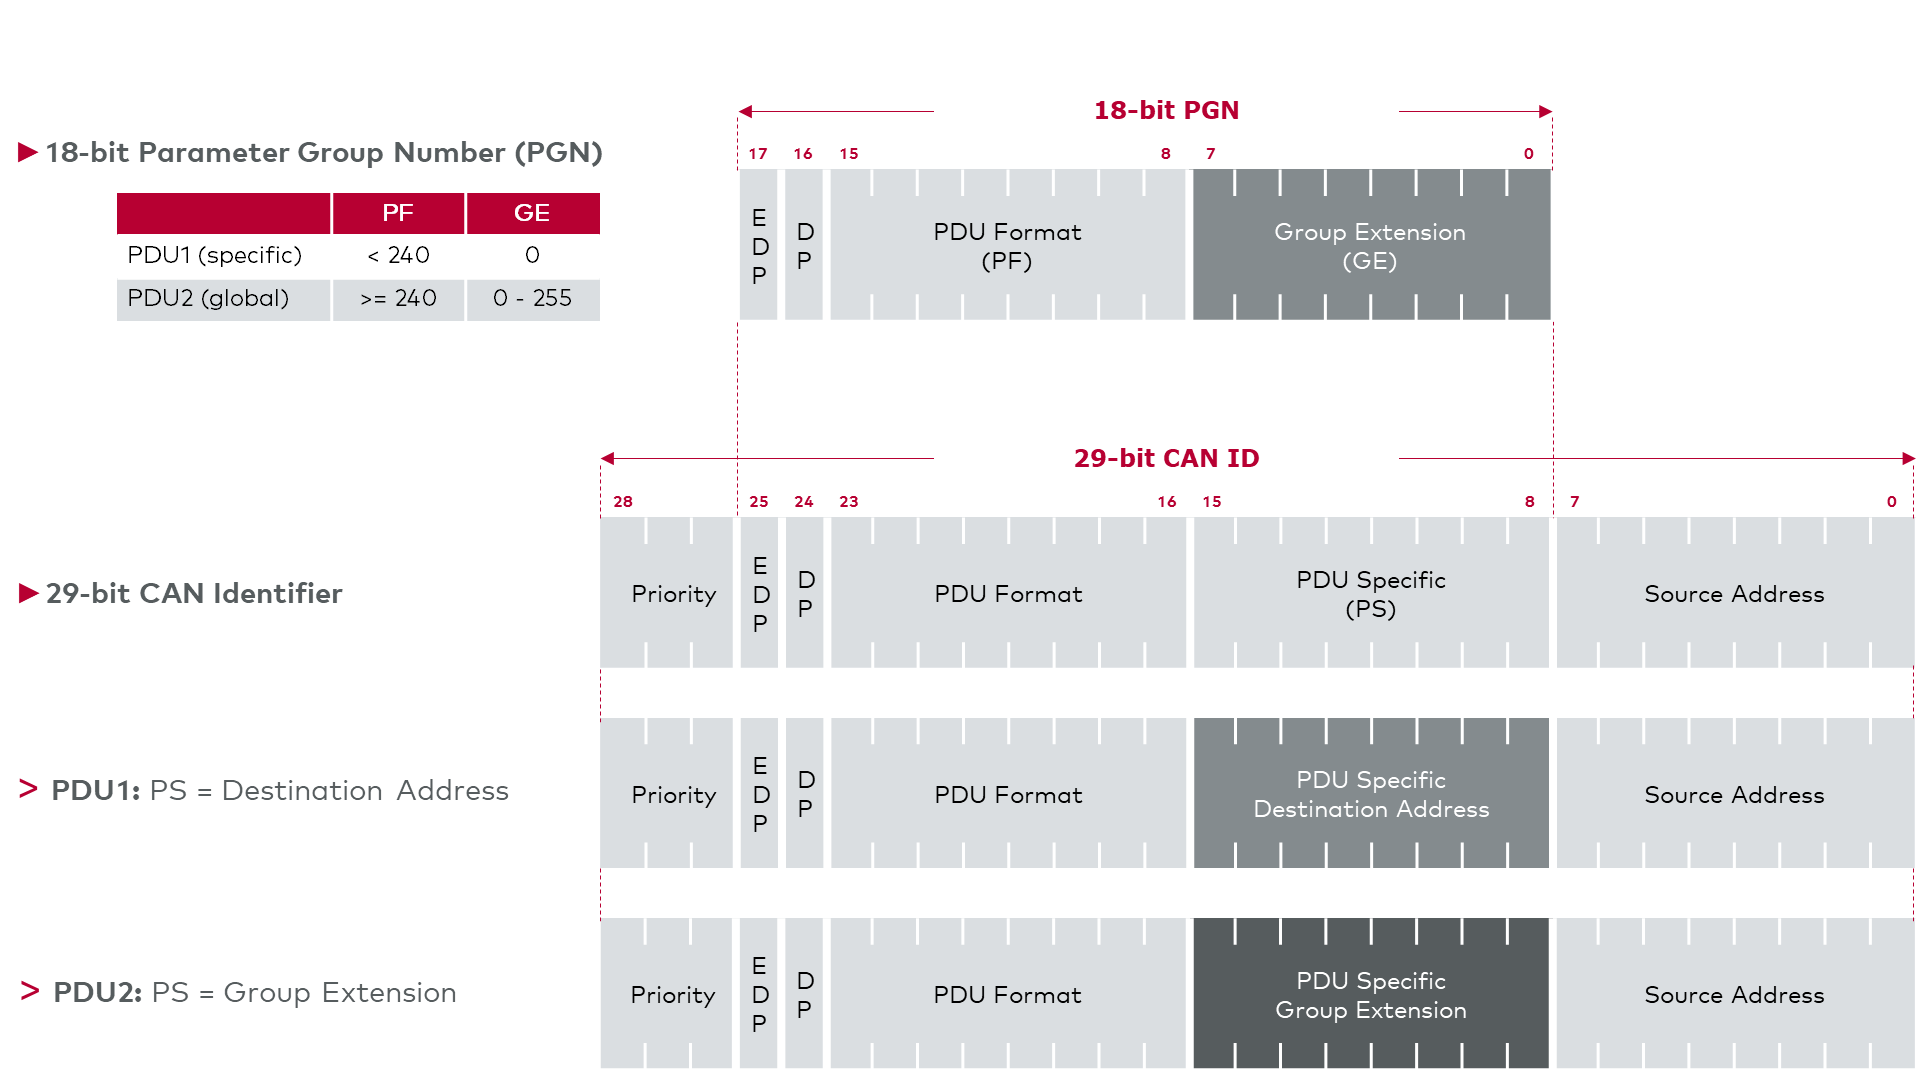
\includegraphics[scale=0.28]{images/j1939header.png}
    \caption{Header einer J1939-Nachricht auf dem CAN-Bus \cite{VectorSAE}(letzter Zugriff: 28.01.2025)}
    \label{fig:j1939header}
\end{figure}

Trotz des Broadcasting-Prinzips soll nicht jede Nachricht von jedem Knoten verarbeitet werden \cite{Murvay2018}.
Die Zieladresse ermöglicht es, dass eine Nachricht nur von dem designierten Knoten verarbeitet wird.
Um eine Nachricht an alle Knoten 
zu senden, wird die Zieladresse auf 255 gesetzt. Mit der Gruppenerweiterung ist es nicht möglich eine Nachricht 
zielgerichtet an bestimmte Geräte zu senden. 




\section{Raspberry Pi}
Ein Raspberry Pi ist ein Einplatinencomputer, der von der Raspberry Pi Foundation entwickelt wurde. 
Dieser hat den Prozessor mit Grafikeinheit, Arbeitsspeicher, Speicher und Anschlüssen auf einem einzigen Board integriert.
Es handelt sich um einen vollwertiger Computer, der kleiner als normale PCs ist. Für die Größe ist der Raspberry Pi
leistungsstark. Zusätzlich kann dieser mit einem normalen Betriebssystem
betrieben werden. Das macht ihn zu einem vielseitigen Werkzeug und attraktiv für diese Arbeit.
Trotzdem gibt es ein spezielles Betriebssystem, das für den Raspberry Pi entwickelt wurde, das Raspberry Pi OS (ehemals Raspbian).
Dieses basiert auf der Linux-Distribution Debian. Um viele Funktionen erfüllen zu können, hat der Raspberry Pi viele Anschlüsse.
Der Raspberry Pi 5 hat 4 USB-Anschlüsse, 2 Micro-HDMI-Anschlüsse, 1 Ethernet-Anschluss, 1 USB-C-Anschluss 
für die Stromversorgung und einen Micro-SD-Kartensteckplatz.

\subsection{Raspberry Pi als Rogue Device}
Unter einem Rogue Device versteht man ein Gerät, das sich unautorisiert und unauffällig in ein Netzwerk integriert \cite{Scarfone2008}.
Dies kann ein Raspberry Pi sein, der sich in ein Netzwerk einbindet und Daten abfängt oder manipuliert. Hierüber können 
sich Angreifer Zugriff auf das Netzwerk verschaffen. 
Ein solches Gerät kann dazu verwendet werden, um eigenen Code auszuführen. Der kann beispielsweise Daten veränden oder 
weitere Angriffe vorbereiten. Zudem kann es von Angreifern aus der Ferne gesteuert werden, wodurch gezielte 
Manipulationen oder Spionageangriffe vereinfacht werden. Darüber hinaus lässt sich ein Rogue Device nutzen, um Informationen 
über das Netzwerk zu sammeln, etwa durch das Mithören von Kommunikation oder die Analyse von Sicherheitsmechanismen.
Das ermöglicht es, Schwachstellen im Netzwerk aufzudecken und gezielt auszunutzen.

\section{State of the Art}
Die Technologie des CAN-Bus ist seit einiger Zeit etabliert und wird in vielen Bereichen eingesetzt.
Daher gibt es auch viele Tools und Bibliotheken, die es ermöglichen, mit dem CAN-Bus zu arbeiten.
In diesem Abschnitt wird der aktuelle Stand der Technik vorgestellt.

\subsection{Anbindung von Raspberry Pi an CanBus}
In der folgenden Arbeit soll ein Raspberry Pi an einen CAN-Bus angeschlossen werden. 
Im Folgenden werden einige verschiede Möglichkeiten vorgestellt.\\
Die erste Möglichkeit ist die Verwendung eines Microchip MCP251x, der als CAN-Controller dient \cite{Salunkhe2016}. Dieser wird 
mit dem Microchip MCP2551 ergänzt, der als CAN-Transceiver dient. Diese Kombination ermöglicht es, den
Raspberry Pi mit dem CAN-Bus zu verbinden. Der MCP251x wird über die SPI-Schnittstelle (Serial Peripheral Interface) 
des Raspberry Pi angeschlossen. Dazu wird ein Treiber benötigt, der die Kommunikation zwischen dem Raspberry Pi und dem
MCP251x ermöglicht. Ein solcher Treiber ist bereits seit dem 05.05.2015 im Raspberry Pi OS (ehemals Raspbian OS)
integriert. 
Um diese Möglichkeit zu vereinfachen, gibt es auch verschiedene HATs (Hardware Attached on Top), die solche Microchips
bereits integriert haben \cite{Pant2019}. Ein Beispiel dafür ist das PiCan2 von SK Pang Electronics. Dieses Board wird auf den 
GPIO-Pins (General Purpose Input/Output) des Raspberry Pi gesteckt. Es erlaubt dem Raspberry Pi mit dem CAN-Bus
zu kommunizieren. Das PiCan2 unterstützt eine Geschwindigkeit von bis zu 1Mbit/s. \\
Es besteht auch die Möglichkeit, einen USB-CAN-Adapter zu verwenden. Damit ist die Anbindung eines 
beliebigen Computer an den CAN-Bus möglich.
Ein Beispiel für einen solchen Adapter ist der UCAN von Fysetc \cite{FysetcUCAN} (letzter Zugriff: 17.02.2025). 
Die Hardware und Firmware des Adapters
sind open-source. Die Verbindung zum Raspberry Pi erfolgt über USB-C.
Zum CAN-Bus müssen lediglich CAN\_H und CAN\_L und die Masse verbunden werden. Mit dem richtigen Treiber funktioniert
dieser Adapter mit Linux, Windows und MacOS.  



\subsection{Überseztung von CAN-Nachrichten}
Viele Software Tools ermöglichen die Arbeit mit dem CAN-Bus. Um einen Überblick zu bekommen, 
werden hier einige vorgestellt. Diese Tools unterscheiden sich in ihrem Funktionsumfang, ihrer Benutzerfreundlichkeit 
und den unterstützten Anwendungsfällen. Einige Programme sind speziell für die Analyse und das Debugging von CAN-Nachrichten 
ausgelegt, während andere umfassende Entwicklungs- und Simulationsmöglichkeiten bieten. Im Folgenden werden die wichtigsten 
Eigenschaften, Einsatzbereiche und Besonderheiten der einzelnen Tools vorgestellt. \\
\begin{itemize}
    \item \textbf{canCommander}: Dieses Tool ermöglicht das Senden und Empfangen von CAN-Nachrichten. Es bietet eine einfache 
    Benutzeroberfläche und umfangreiche Analysefunktionen. Mit canCommander können CAN-Nachrichten aufgezeichnet, 
    analysiert und bearbeitet werden. Dabei können auch Nachrichten gesendet und injiziert werden. Es wird auch eine
    schon vorbereitete Platine verkauft, die es ermöglicht, mit dem CAN-Bus zu arbeiten. Dennoch ist canCommander ein
    open-source Projekt und kann auch auf anderen Plattformen verwendet werden. Diese Plattformen beschränken sich aber
    auf Mikrocontroller, wie Arduino Uno oder ESP32. \cite{can_commander} (letzter Zugriff: 15.02.2025)
    \item \textbf{cantools}: Diese Python-Bibliothek ermöglicht es, CAN-Nachrichten zu dekodieren. Mit cantools können 
    CAN-Daten in ein Menschenlesbares Format umgewandelt werden. Die Bibliothek 
    bietet eine Vielzahl von Funktionen und unterstützt verschiedene Protokolle und Datenformate. Damit ist cantools ist ein 
    nützliches Werkzeug für die Analyse und Verarbeitung von CAN-Nachrichten und eignet sich für die Entwicklung von 
    Anwendungen, die mit dem CAN-Bus arbeiten. \cite{cantools} (letzter Zugriff: 15.02.2025)
    \item \textbf{CANoe}: Dieses eigenständige kommerzielle Tool wurde von der Firma Vector Informatik GmbH. entwickelt.
    Es bietet eine vielzahl an verschiedenen Funktionen. CANoe ermöglicht die Entwicklung, Simulation und Analyse von
    CAN-Netzwerken. Es bietet eine umfangreiche Funktionalität und unterstützt verschiedene Protokolle und Datenformate.
    \cite{VectorCANoe} (letzter Zugriff: 15.02.2025)
    \item \textbf{can\_decoder}: Das Open-Source-Projekt ermöglicht das Dekodieren von CAN-Nachrichten. Es wurde von der Firma
    CSS-Electronics entwickelt und ist auf GitHub verfügbar. Allerdings ist das Projekt nicht mehr aktiv und wird nicht mehr
    weiterentwickelt. Trotzdem kann es ein nützliches Werkzeug für die Analyse und Verarbeitung von CAN-Nachrichten sein. 
    \cite{can_decoder} (letzter Zugriff: 15.02.2025)
    \item \textbf{SavvyCAN}: Die C++ Anwendung kann CAN-Nachrichten aufzeichnen, welche durch Reverse-Engineering analysiert werden können.
    Hiermit können auch einzelne Nachrichten dekodiert werden. SavvyCAN ist ein Open-Source-Projekt und kann auf GitHub gefunden werden. Zusätzlich
    gibt es Unterstützung auf Linux und Windows. \cite{SavvyCAN} (letzter Zugriff: 15.02.2025)
    \item \textbf{can-utils}: Diese Set an Linux-Tools ermöglichen die Arbeit mit dem CAN-Bus. Damit ist es möglich, CAN-Nachrichten zu senden und zu empfangen.
    Es ist ein Open-Source-Projekt und kann auf GitHub gefunden werden. Diese Tools bieten eine Grundlage für die Entwicklung von Anwendungen, die mit dem CAN-Bus arbeiten.
    \cite{can-utils} (letzter Zugriff: 15.02.2025)
\end{itemize}
Um der Nutzlast der CAN-Bus Nachrichten Informationen zuzuordnen, ist eine DBC-Datei essentiell \cite{Choi2021}. 
Diese Datei schlüsselt auf, welche Informationen in den verschiedenen CAN-Nachrichten enthalten sind.
Da auch sensible Informationen in den Nachrichten enthalten sein können, wird diese Datei in den meisten 
Fällen nicht öffentlich verfügbar gemacht. Ohne diese Datei können zwar Brute-Force Ansätze verwendet werden,
allerdings ist dies sehr aufwendig und nicht zielführend. \\
Um die vorher genannten Tools zu verwenden, ist es also notwendig, die DBC-Datei zu haben. Bei canCommander
sind einige DBC-Dateien bereits vorinstalliert. Bei cantools kann die DBC-Datei in das Programm geladen werden.
Allerdings kann es eine Schwierigkeit darstellen, die bestimmte DBC-Datei zu erhalten.
\clearpage
\chapter{State of the Art}
\printmyminitoc{1}

Für eine Sicherheitsanalyse von maritimen Steuerungssystemen ist es wichtig, die aktuelle Technik und die
Möglichkeiten von Angreifern zu kennen. In diesem Kapitel wird der aktuelle Stand der Technik vorgestellt.
Der Fokus liegt dabei auf Technologien, die für die Arbeit relevant sind.

\section{Rogue Device}
Unter einem Rogue Device versteht man ein Gerät, das sich unautorisiert und unauffällig in ein Netzwerk integriert \cite{Scarfone2008}.
Dies kann ein Raspberry Pi sein, der sich in ein Netzwerk einbindet und Daten abfängt oder manipuliert. Hierüber können 
sich Angreifer Zugriff auf das Netzwerk verschaffen. 
Ein solches Gerät kann dazu verwendet werden, um eigenen Code auszuführen. Der kann beispielsweise Daten veränden oder 
weitere Angriffe vorbereiten. Zudem kann es von Angreifern aus der Ferne gesteuert werden, wodurch gezielte 
Manipulationen oder Spionageangriffe vereinfacht werden. Darüber hinaus lässt sich ein Rogue Device nutzen, um Informationen 
über das Netzwerk zu sammeln, etwa durch das Mithören von Kommunikation oder die Analyse von Sicherheitsmechanismen.
Das ermöglicht es, Schwachstellen im Netzwerk aufzudecken und gezielt auszunutzen.

\subsection{Angriff mit einem Rogue Device}

\section{Arbeit mit dem CAN-Bus}
Die Technologie des CAN-Bus wird in vielen Bereichen eingesetzt.
Daher gibt es auch viele Tools und Bibliotheken, die es ermöglichen, mit dem CAN-Bus zu arbeiten.
In diesem Abschnitt wird der aktuelle Stand der Technik vorgestellt.

\subsection{Anbindung von Raspberry Pi an CAN-Bus} \label{sec:raspberryPiToCAN}	
In der folgenden Arbeit soll ein Raspberry Pi an einen CAN-Bus angeschlossen werden. 
Im Folgenden werden einige verschiede Möglichkeiten vorgestellt.\\
Die erste Möglichkeit ist die Verwendung eines Microchip MCP251x, der als CAN-Controller dient \cite{Salunkhe2016}. Dieser wird 
mit dem Microchip MCP2551 ergänzt, der als CAN-Transceiver dient. Diese Kombination ermöglicht es, den
Raspberry Pi mit dem CAN-Bus zu verbinden. Der MCP251x wird über die SPI-Schnittstelle (Serial Peripheral Interface) 
des Raspberry Pi angeschlossen. Dazu wird ein Treiber benötigt, der die Kommunikation zwischen dem Raspberry Pi und dem
MCP251x ermöglicht. Ein solcher Treiber ist bereits seit dem 05.05.2015 im Raspberry Pi OS (ehemals Raspbian OS)
integriert \cite{Salunkhe2016}. 
Um diese Möglichkeit zu vereinfachen, gibt es auch verschiedene HATs (Hardware Attached on Top), die solche Microchips
bereits integriert haben \cite{Pant2019}. Ein Beispiel dafür ist das PiCan2 von SK Pang Electronics. Dieses Board wird auf den 
GPIO-Pins (General Purpose Input/Output) des Raspberry Pi gesteckt. Es erlaubt dem Raspberry Pi mit dem CAN-Bus
zu kommunizieren. Das PiCan2 unterstützt eine Geschwindigkeit von bis zu 1Mbit/s. \\
Es besteht auch die Möglichkeit, einen USB-CAN-Adapter zu verwenden. Damit ist die Anbindung eines 
beliebigen Computer an den CAN-Bus möglich.
Ein Beispiel für einen solchen Adapter ist der UCAN von Fysetc \cite{FysetcUCAN}. 
Die Hardware und Firmware des Adapters
sind open-source. Die Verbindung zum Raspberry Pi erfolgt über USB-C.
Zum CAN-Bus müssen lediglich CAN\_H und CAN\_L und die Masse verbunden werden. Da CAN-Bus Treiber für Linux, Windows und Mac
vorhanden sind, kann der UCAN mit diesen Betriebssystemen verwendet werden. 



\subsection{Übersetzung von CAN-Nachrichten} \label{sec:canTranslation}
Viele Software Tools ermöglichen die Arbeit mit dem CAN-Bus. Diese Tools unterscheiden sich in ihrem Funktionsumfang
und den Anwendungsbereichen.
Einige Programme sind speziell für die Analyse und das Debugging von CAN-Nachrichten 
ausgelegt, während andere umfassende Entwicklungs- und Simulationsmöglichkeiten bieten. Im Folgenden werden die wichtigsten 
Eigenschaften, Einsatzbereiche und Besonderheiten der einzelnen Tools vorgestellt. \\
\begin{itemize}
    \item \textbf{canCommander}: Dieses Tool ermöglicht das Senden und Empfangen von CAN-Nachrichten. Es bietet eine einfache 
    Benutzeroberfläche und umfangreiche Analysefunktionen. Mit canCommander können CAN-Nachrichten aufgezeichnet, 
    analysiert und bearbeitet werden. Dabei können auch Nachrichten gesendet und injiziert werden. Es wird auch eine
    schon vorbereitete Platine verkauft, die es ermöglicht, mit dem CAN-Bus zu arbeiten. Dennoch ist canCommander ein
    open-source Projekt und kann auch auf anderen Plattformen verwendet werden. Diese Plattformen beschränken sich aber
    auf Mikrocontroller, wie Arduino Uno oder 
    ESP32.\footnote{\href{https://github.com/MatthewKuKanich/CAN_Commander}{CAN Commander} (besucht am 15.02.2025)}
    \item \textbf{cantools}: Diese Python-Bibliothek ermöglicht es, CAN-Nachrichten zu dekodieren. Mit cantools können 
    CAN-Daten in ein Menschenlesbares Format umgewandelt werden. Die Bibliothek 
    bietet eine Vielzahl von Funktionen und unterstützt verschiedene Protokolle und Datenformate. Damit ist cantools ist ein 
    nützliches Werkzeug für die Analyse und Verarbeitung von CAN-Nachrichten und eignet sich für die Entwicklung von 
    Anwendungen, die mit dem CAN-Bus arbeiten.\footnote{\href{https://github.com/cantools/cantools/releases}{cantools} (besucht am 15.02.2025)}
    \item \textbf{CANoe}: Dieses eigenständige kommerzielle Tool wurde von der Firma Vector Informatik GmbH. entwickelt.
    Es bietet eine vielzahl an verschiedenen Funktionen. CANoe ermöglicht die Entwicklung, Simulation und Analyse von
    CAN-Netzwerken. Es unterstützt verschiedene Protokolle und 
    Datenformate.\footnote{\href{https://www.vector.com/de/de/produkte/produkte-a-z/software/canoe/}{CANoe} (besucht am 15.02.2025)}
    \item \textbf{can\_decoder}: Das Open-Source-Projekt ermöglicht das Dekodieren von CAN-Nachrichten. Es wurde von der Firma
    CSS-Electronics entwickelt und ist auf GitHub verfügbar. Allerdings ist das Projekt nicht mehr aktiv und wird nicht mehr
    weiterentwickelt. Trotzdem kann es ein nützliches Werkzeug für die Analyse und Verarbeitung von CAN-Nachrichten 
    sein.\footnote{\href{https://github.com/CSS-Electronics/can_decoder}{can\_decoder} (besucht am 15.02.2025)}
    \item \textbf{SavvyCAN}: Die C++ Anwendung kann CAN-Nachrichten aufzeichnen, welche zum Reverse-Engineering genutzt werden können.
    Hiermit können auch einzelne Nachrichten dekodiert werden. SavvyCAN ist ein Open-Source-Projekt und kann auf GitHub gefunden werden. 
    Zusätzlich gibt es Unterstützung auf Linux und Windows.\footnote{\href{https://savvycan.com/index.php}{SavvyCAN} (besucht am 15.02.2025)}
    \item \textbf{can-utils}: Diese Set an Linux-Tools ermöglichen die Arbeit mit dem CAN-Bus. Damit ist es möglich, CAN-Nachrichten 
    zu senden und zu empfangen.
    Es ist ein Open-Source-Projekt und kann auf GitHub gefunden werden. Diese Tools bieten eine Grundlage für die Entwicklung von 
    Anwendungen, die mit dem CAN-Bus arbeiten.\footnote{\href{https://github.com/linux-can/can-utils}{can-utils} (besucht am 15.02.2025)}
\end{itemize}
Es ist essentiell die Nutzlast der CAN-Bus Nachrichten Informationen zuzuordnen. Das kann in der Form einer DBC-Datei geschehen\cite{Choi2021}. 
Diese Datei schlüsselt auf, welche Informationen in den verschiedenen CAN-Nachrichten enthalten sind.
Da auch sensible Informationen in den Nachrichten enthalten sein können, wird diese Datei in den meisten 
Fällen nicht öffentlich verfügbar gemacht. Ohne diese Datei können zwar Brute-Force Ansätze verwendet werden,
allerdings ist dies sehr aufwendig und nicht zielführend. \\
Um die vorher genannten Tools zu verwenden, sind DBC-Dateien notwendig, um die zu dekodierenden und kodierenden Nachrichten zu beschreiben. 
Bei canCommander
sind einige DBC-Dateien bereits vorinstalliert. Bei cantools kann die DBC-Datei in das Programm geladen werden.
\begin{figure}[H]
    \centering
    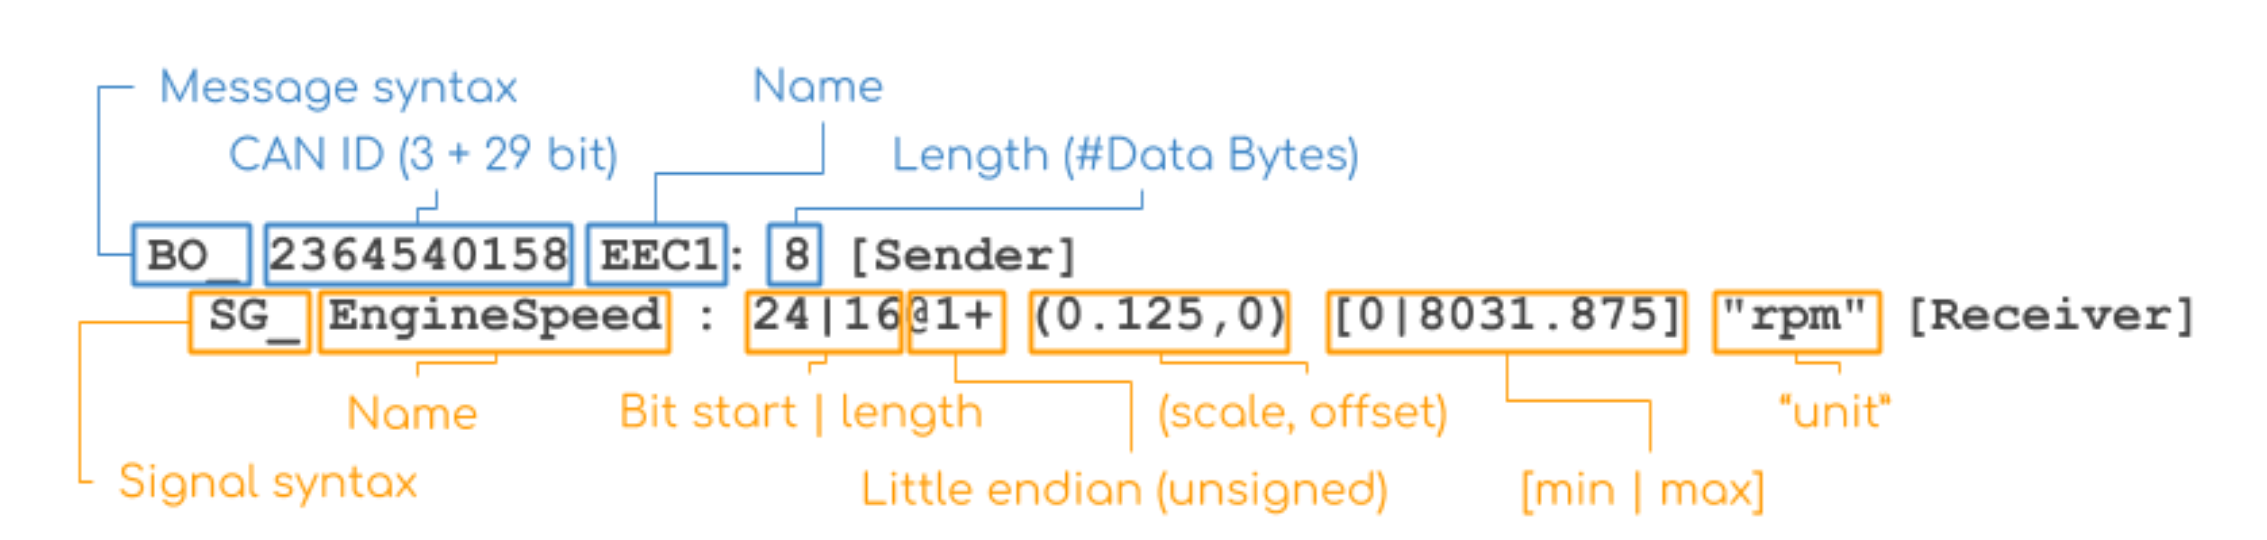
\includegraphics[scale=0.2]{images/CAN-DBC-File-Format-Explained-Intro-Basics_2.png}
    \caption{Auszug aus einer Beispiel DBC-Datei \cite{cssElectronics}}
    \label{fig:dbcfile}
\end{figure}
In Abbildung \ref{fig:dbcfile} ist ein Ausschnitt aus einer DBC-Datei zu sehen.
In dieser sind einzelne Nachrichten aufgelistet. Jede Nachricht hat eine ID, eine Länge und Signale. Diese Signale
haben eine Länge, einen Offset und einen Faktor. Die Signale sind die eigentlichen Informationen, die in den CAN-Nachrichten
kodiert sind. Sie stellen also die Nutzlast der Nachrichten dar. Mit diesen Informationen kann eine Nachricht erstellt werden.
Im Anschluss an die Nachrichtentypen werden in der DBC-Datei für bestimmte Signale die möglichen Eingaben definiert.
Das hilft bei der richtigen Wahl der Eingabe. 
\clearpage
\chapter{Konzept und Systemdesign}
\printmyminitoc{1}

\section{Aufbau Schiffsysteme}
Wie werden die Motoren im Schiff angesteuert?
Welche Angriffsmöglichkeiten gibt es?
Wie wird das Ruder angesteuert?
Gibt es noch weitere wichtige Systeme?
\begin{itemize}
    \item einzelnen Can-Bus für jeden Gashebel
    \item Serielle Kommunikation bei Autopilot
    \item Autopilot kann nur das Ruder steuern
\end{itemize}

\section{Steuerungslogik des Controllers}
Der benutzte Controller ist ein Xbox Series X Controller. Dieser wurde gewählt, da er eine gute Haptik hat und weit
verbreitet ist. Zusätzlich ist er kabellos und kann somit frei bewegt werden. Um die Steuerung des Schiffes zu
ermöglichen, müssen die Eingaben des Controllers in Steuerbefehle umgewandelt werden. Dies passiert auf dem 
Raspberry Pi. Der Controller wird über Bluetooth mit dem Raspberry Pi verbunden. Dort werden die Eingaben des Controllers
ausgelesen und in einem Python-Programm in Steuerbefehle umgewandelt. \\
Um eine einfache Steuerung zu ermöglichen, wird im folgenden die Tastenbelegung aufgeschlüsselt.
Um alle gewünschten Funktionen umzusetzen, werden nicht alle Tasten benötigt. 

\begin{figure}[H]
    \centering
    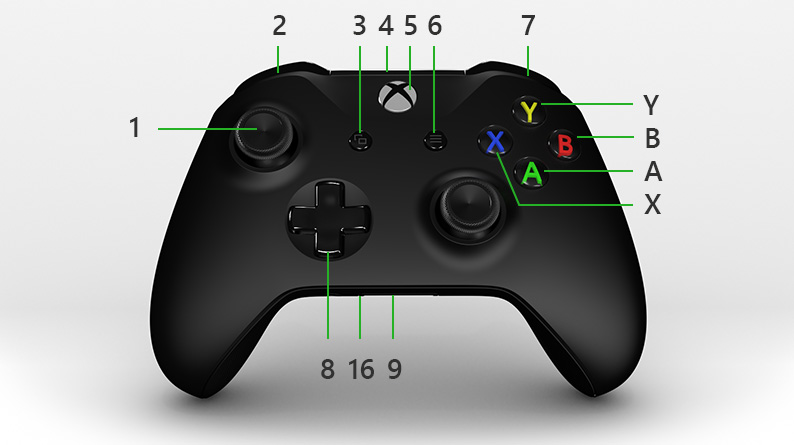
\includegraphics[scale=0.5]{images/vorderseite.jpg}
    \caption{Vorderseite des Controllers \cite{XboxController}(letzter Zugriff: 24.01.2025)}
    \label{fig:vorderseite}
\end{figure}

\begin{figure}[H]
    \centering
    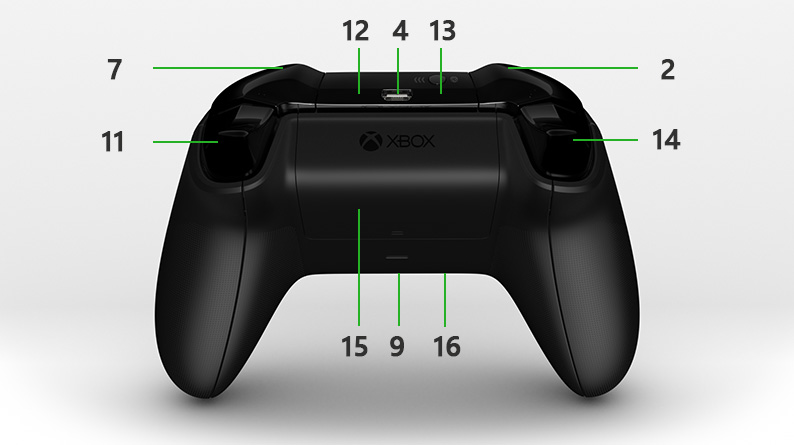
\includegraphics[scale=0.5]{images/rueckseite.jpg}
    \caption{Rückseite des Controllers \cite{XboxController}(letzter Zugriff: 24.01.2025)}
    \label{fig:rueckseite}
\end{figure}

\begin{table}[H]
    \begin{tabular}{|c|c|}
    \hline
    \rowcolor[gray]{0.8}
     Nummerierung der Taste & Funktion \\ \hline 
     1 & Bewegung des Ruders \\ \hline 
     2 & Reduzierung der linken Gashebelposition \\ \hline 
     7 & Reduzierung der rechten Gashebelposition \\ \hline
     11 & Erhöhung der rechten Gashebelposition \\ \hline
     14 & Erhöhung der linken Gashebelposition \\ \hline
     B + 2 & Umschalten des Rückwärtsgangs am linken Motor \\ \hline
     B + 7 & Umschalten des Rückwärtsgangs am rechten Motor \\ \hline
     B + 2 + 7 & Umschalten des Rückwärtsgangs an beiden Motoren \\
      & (basierend auf dem derzeitigen Gang am rechten Motor) \\ \hline
    \end{tabular}
\end{table}
Das Einlegen des Rückwärtsgangs ist durch eine Tastenkombination so gewählt, dass es nicht aus Versehen passieren kann.
Mit jeweils der Taste 2 oder 7 wird die Gashebelposition reduziert. Mit der zusätzlichen Betätigung der Taste B wird der 
Rückwärtsgang eingelegt an dem jeweiligen Motor. Wenn die Tasten 2, 7 und B gleichzeitig betätigt werden, 
wird der Rückwärtsgang für beide Motoren gleichzeitig umgeschalten. Dies ist so gewählt, da eine Verzögerung bei dem
Umschalten eines Rückwärtsgangs von 10 Sekunden eingebaut ist. Das soll dem Getriebe ermöglichen, den Gang zu wechseln
ohne eine direkte Gaseingabe. Nun muss es aber auch möglich sein, beide Rückwärtsgänge gleichzeitig umzuschalten, daher 
die vergleichsweise komplexe Tastenkombination.



\section{Integration des Rogue Device}
Damit der Controller die Steuerbefehle an das Schiff senden kann, muss das Rogue Device in das System integriert werden.
In diesem Fall ist das Rogue Device der Raspberry Pi. Damit dieser möglichst unbemerkt in das System integriert werden könnte,
muss der Controller drahtlos verbunden werden. Um die Kommunikation von dem Rogue Device zu dem Schiff zu ermöglichen, müssen
die einzelnen Systeme angesteuert werden. Um die Gashebelposition zu verändern, wird der Raspberry Pi mit dem Can-Bus des Schiffes
verbunden. 
\begin{itemize}
    \item Stromversorgung des Raspberry Pi (Battery Pack oder Steckdose)
\end{itemize}

Sollte der Gashebel in der normalen Benutzung vom Schiffsführer benutzt werden, wird ein Signal an den Can-Bus gesendet. Dieses Signal wird dann an die Motoren weitergeleitet.
Um diese Eingabe zu verhindern, muss auf diese Nachricht geachtet und reagiert werden. Mit dem Lesen des Can-Bus kann die 
entsprechende Nachricht entdeckt werden. Dann kann eine Nachricht von dem Rogue Device gesendet werden, um die Gashebelposition
zu überschreiben.
\\
Um eine Rückmeldung zu erhalten, wie die gewünschte Gashebel- und Ruderposition ist, sollte mit einer einfachen App
gearbeitet werden. Diese App kann dann die gewünschten Positionen anzeigen. Ein kleiner OLED-Bildschirm könnte auch benutzt 
werden. Allerdings hat dieser den Nachteil, dass er physisch an den Raspberry Pi angeschlossen werden muss. Damit 
ist keine Rückmeldung möglich, wenn dieser als Rogue Device in dem System versteckt angeschlossen ist.
Um die Kommunikation zwischen dem Raspberry Pi und dem Handy mit der App zu ermöglichen, wird Bluetooth benutzt.


Wie in der Abbildung \ref{fig:j1939header} zu sehen, besteht der Header aus einer PGN, einer Quelladresse und einer Priorität. Um nun Nachrichten
an den Motor zu senden, kann eine Nachricht des Gashebels abgefangen werden. Die PGN kann für die eigene Nachricht genutzt
werden. Die Quelladresse kann man auch kopieren. Die Priorität sollte möglichst klein gewählt werden, 
damit die eigene Nachricht bevorzugt wird. In der eigenen Nachricht kann dann die gewünschte Gashebelposition gesendet werden.

\subsection{Rückmeldung der Eingaben}
\begin{itemize}
    \item Was passiert bei Veränderung der Gashebelposition?
    \item Wie passiert die Rückmeldung
    \item wichtig um pilot induced oscillation zu verhindern
\end{itemize}
Was muss ich dabei beachten?
Muss eine Rückmeldung für die Eingaben geschehen? Wenn ja, wie?
(kleiner OLED-Bildschirm oder App)
Es muss eine Art der Rückmeldung geben, um in etwa die Eingaben im Vergleich zum momentanen Zustand zu sehen.
Dabei sollte die Rückmeldung möglichst unauffällig sein. Ein kleiner OLED-Bildschirm könnte benutzt werden, allerdings
muss dieser physisch an den Raspberry Pi angeschlossen werden. Das würde die Versteckung des Rogue Devices erschweren.
Eine App auf einem Handy könnte die Rückmeldung geben. Diese App könnte dann die gewünschten Positionen anzeigen.
Dafür muss der Raspberry Pi mit dem Handy verbunden werden. Dies könnte über Bluetooth geschehen.
Hier ist zu beachten, dass die Verbindung stabil ist und nicht von anderen Geräten gestört wird.
Jedoch kann ist hier mit einem größeren Aufwand zu rechnen, da die App erst entwickelt werden muss.
Eine weitere Möglichkeit würden Vibrationen im Xbox Controller sein. Diese könnten genutzt werden, wenn die derzeitige
Eingabe ein Maximum oder Minimum erreicht hat. Allerdings ist dies nicht so genau wie eine Anzeige auf einem Bildschirm.
Es könnten auch nur wenige bestimmte Positionen mittgeteilt werden.
\clearpage
\chapter{Implementierung}
\printmyminitoc{1}

In diesem Kapitel wird die Implementierung des Rogue Devices beschrieben. Dabei wird auf die Verbindung des Rogue Devices
mit dem Controller und dem Schiff eingegangen. Zudem wird die Umsetzung der Kommunikation zwischen den einzelnen Komponenten
beschrieben. Dabei hat die Übersetzung von CAN-Bus Nachrichten eine wichtige Rolle gespielt.

\section{Umsetzung des Rogue Device}
Wie bereits in Kapitel \ref{sec:raspberrypi} beschrieben, wird ein Raspberry Pi 5 als Rogue Device benutzt. 
Als Betriebssystem wird Raspberry Pi OS benutzt. Der Standard Package Manager ist APT. Unter dessen Benutzung werden 
Python 3.12 und die benötigten Bibliotheken installiert. Damit sind die Vorraussetzungen für die weitere Implementierung
gesetzt.

\section{Verbindung Rogue Device - Controller} 

Im ersten Schritt wird der Spiele-Controller mit dem Raspberry Pi verbunden. Der Raspberry Pi wird mit Raspberry Pi OS betrieben.
Als Standard-Bluetooth-Treiber wird BlueZ\footnote{\href{https://www.bluez.org/}{BlueZ} (besucht am 02.01.2025)} verwendet. 
Dieser ist bereits vorinstalliert und muss 
nicht manuell installiert werden. Da es sich in diesem Fall um einen Xbox-Controllers handelt, wurde der Treiber
xboxdrv\footnote{\href{https://github.com/xboxdrv/xboxdrv}{xboxdrv} (besucht am 02.01.2025)} installiert. 
Diese können im APT-Repository gefunden werden.
Zusätzlich muss der Enhanced Re-Transmission Mode (ERTM) deaktiviert 
werden.\footnote{\href{https://wiki.debian.org/Gamepad\#Xbox\_Controllers\_over\_Bluetooth}{Debian Wiki} (besucht am 22.03.2025)} 
Dieser Modus ist standardmäßig aktiviert und
verhindert die korrekte Verbindung des Controllers, aufgrund eines Kompatibilitätsproblem.
Zusätzlich muss sichergestellt werden, dass die Firmware des Spiele-Controllers
auf dem aktuellen Stand ist. Um den Xbox-Controller zu verbinden, kann die graphische Benutzeroberfläche benutzt werden.
\\
Als Programmiersprache wird Python 3 benutzt. Die Sprache wurde gewählt, da für alle benötigten Funktionen bereits eine Bibliothek
existiert.
Die Struktur des Rogue Devices soll wie folgt aussehen:
\begin{figure}[H]
    \centering
    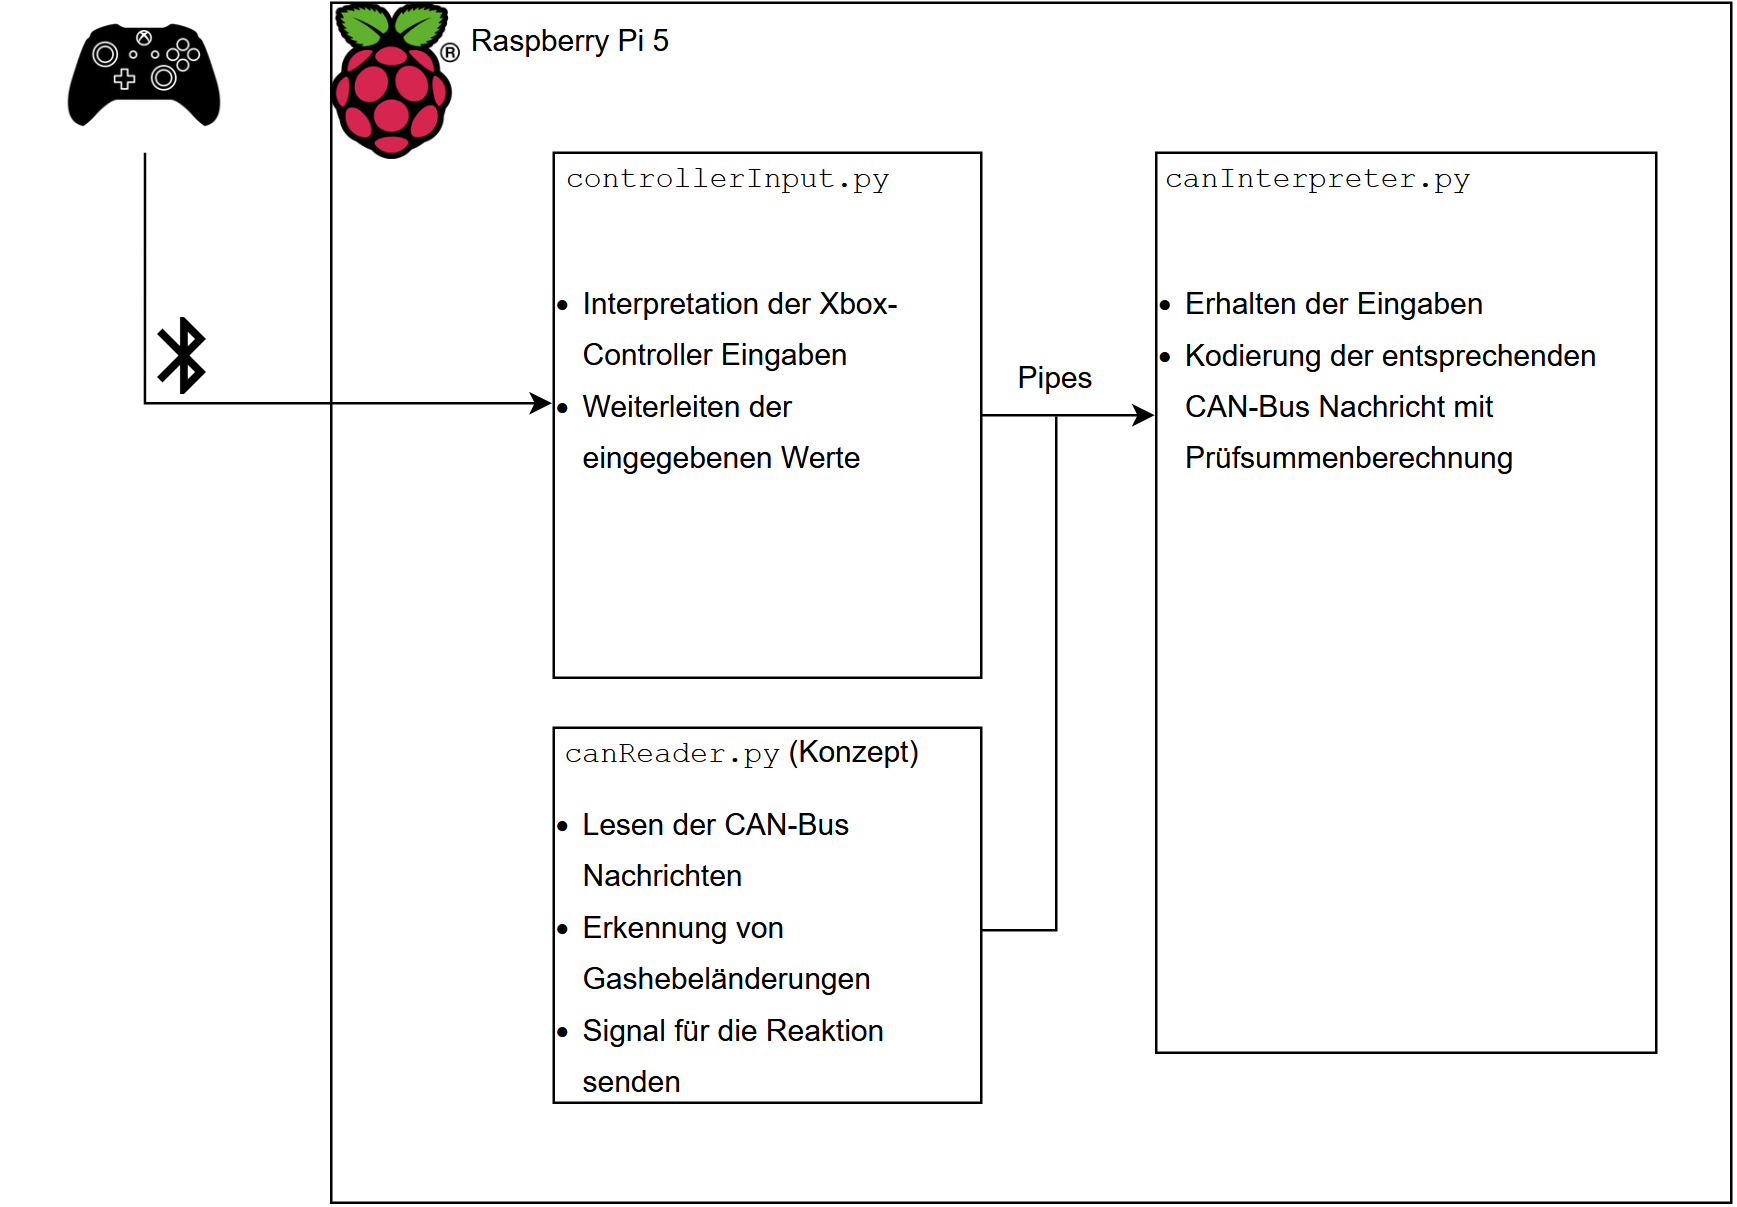
\includegraphics[scale=0.4]{images/piKonzept.png}
    \caption{Programmstruktur auf dem Rogue Device}
    \label{fig:structureRogueDevice}
\end{figure}

Für das im Rahmen der Arbeit entwickelte Programm \texttt{controllerInput.py} wird die Bibliothek \texttt{pygame} benutzt.
Eine Einordnung des entwickelten Programms in die Programmstruktur ist in Abbildung \ref{fig:structureRogueDevice} zu sehen.
Die Bibliothek ermöglicht es, Eingaben von einem Controller zu empfangen. Diese Eingaben
werden in Variablen gespeichert. Dabei gilt es zu beachten, dass der Gashebel oder die Ruderposition nicht
zu schnell verändert werden. Dies könnte zu einem unkontrollierten Verhalten des Schiffes oder zu Schäden führen. 
Daher werden diese Werte mit Tasten des
Controllers eingegeben, welche nicht nur eine binäre Eingabe haben. Diese werden als Achsen bezeichnet. Diese ermöglichen
eine stufenlose Eingabe. Bei einer vollständigen Eingabe soll die Gashebelposition nach 20 Sekunden 100\% erreichen.
So ist sichergestellt, dass die Gashebelposition nicht zu schnell verändert wird. Die Ruderposition soll nach 2 Sekunden
in jede Richtung jeweils 100\% erreichen. Dies ist ein Kompromiss zwischen Geschwindigkeit und Genauigkeit.

\section{Übersetzung Signale Controller - Schiff} \label{sec:signalControllerSchiff}

Wie in Abbildung \ref{fig:structureRogueDevice} zu sehen ist, erhält \texttt{controllerInput.py} die Signale des Xbox-Controllers 
erhält Variablen in Python interpretiert.
Diese Variablen müssen
dann in Nachrichten für den CAN-Bus umgewandelt werden. Hierfür wurde ein weiteres Programm entwickelt, welches die Übersetzung die 
Kodierung der CAN-Bus Nachrichten realisiert. Dieses Programm wird \texttt{canInterpreter.py} genannt.
Damit die beiden Programme miteinander kommunizieren
können, wird Inter-Process-Communication (IPC) benutzt. Als Methode werden hierbei Pipes benutzt. Diese sind einfach zu implementieren und haben
eine automatische Synchronisierung zwischen den Prozessen. Dadurch müssen Prozesse nicht aufeinander warten und können weiterarbeiten. 
Die Synchronisierung wird durch den Puffer der Pipe sichergestellt \cite{Venkataraman2015}. 
Wenn dieser voll ist, wird der schreibende Prozess angehalten, bis der
lesende Prozess den Puffer geleert hat. Dies ist ein einfaches und effizientes Verfahren, 
um die beiden Prozesse zu synchronisieren. Im Rahmen dieser Arbeit dafür ein weiteres Programm entwickelt, welches die Kommunikation
zwischen \texttt{controllerInput.py} und \texttt{canInterpreter.py} ermöglicht. Dieses Programm wird \texttt{mainProcess.py} genannt und 
benutzt die Bibliothek \texttt{subprocess}. Dabei werden die beiden Prozesse als Subprozesse gestartet. Die Ausgaben von 
\texttt{controllerInput.py} werden in die Pipe geschrieben und von \texttt{canInterpreter.py} als Eingaben gelesen.

\subsection{Eingabe-Interface}
Durch die begrenzte Zeit dieser Arbeit, wurde die Rückmeldung mit Vibrationen im Xbox-Controller implementiert.
Dabei wird bei Erreichen des Maximums oder Minimums der Gashebelposition eine Vibration ausgelöst. Das ist eine einfache
Methode, um dem Benutzer eine Rückmeldung zu geben. Auch bei der hälfte der Gashebelposition wird eine kurze und leichte 
Vibration ausgelöst. Das soll ermöglichen, dass es eine ungefähre Vorstellung der Gashebelposition gibt.
Bei der Ruderposition wird eine Vibration ausgelöst, wenn die Ruderposition 100\% erreicht hat in jeweils beide Richtungen
erreicht hat. Bei der Mitte der Ruderposition wird eine kurze und leichte Vibration ausgelöst. Wenn die 
Ruderposition auf 50\% in eine Richtung ist, werden zwei kurze und leichte Vibrationen ausgelöst. Das soll die Bedienung
erleichtern. Die Bedienung von Gashebel und Ruderposition soll dabei möglichst getrennt voneinander vorgenommen werden.
\\
Die Ruderstellung wird durch den linken Stick des Controllers gesteuert. Wenn die Eingabe eine bestimmte Schwelle überschreitet,
wird dies wie Folgt durch Vibrationen signalisiert: 
\begin{figure}[H]
    \centering
    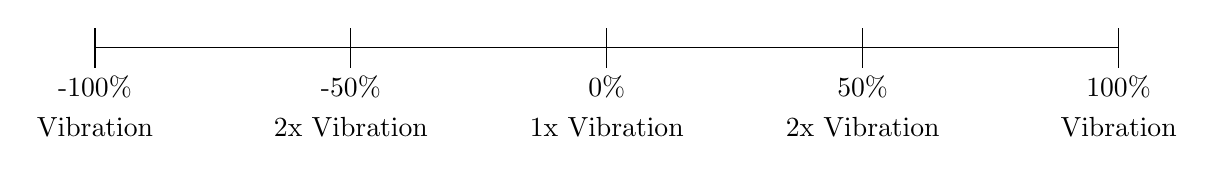
\begin{tikzpicture}
        \draw (0,0) -- (13,0);
        \draw (0,0.25) -- (0,-0.25);
        \draw (0,-0.5) node {-100\%};
        \draw (0,-1) node {Vibration};
        \draw (3.25, 0.25) -- (3.25, -0.25);
        \draw (3.25,-0.5) node {-50\%};
        \draw (3.25,-1) node {2x Vibration};
        \draw (6.5,0.25) -- (6.5,-0.25);
        \draw (6.5,-0.5) node {0\%};
        \draw (6.5,-1) node {1x Vibration};
        \draw (9.75,0.25) -- (9.75,-0.25);
        \draw (9.75,-0.5) node {50\%};
        \draw (9.75,-1) node {2x Vibration};
        \draw (13,0.25) -- (13,-0.25);
        \draw (13,-0.5) node {100\%};
        \draw (13,-1) node {Vibration};
    \end{tikzpicture}
\end{figure}

Dabei ist die Schwelle so gewählt, dass die Vibrationen nicht zu oft ausgelöst werden. 
Es ist wichtig zu wissen, dass der Wert basierend auf der Eingabe des Joysticks kontinuierlich berechnet wird.
Die Eingabe beträgt -1 bis 1. Dabei ist -1 die maximale Position nach links und 1 die maximale Position nach rechts.
Damit die Ruderstellung nicht zu schnell verändert wird, benötigt diese eine volle Eingabe von 1 oder -1 für 2 Sekunden,
damit die Ruderstellung 100\% erreicht. Entsprechend werden die 100\% langsamer erreicht, wenn die Eingabe geringer
ist.

\subsection{CAN-Bus Nachrichtenkodierung} \label{sec:canBus}
Die Kodierung der CAN-Bus Nachrichten ist der Hauptbestandteil des Programms \texttt{canInterpreter.py}, welches im Rahmen dieser Arbeit
entwickelt wurde. 
Das Teilprogramm \texttt{canInterpreter.py} erhält Eingaben von \texttt{controllerInput.py}. Basierend auf den
Eingaben des Xbox-Controllers wird dann die entsprechende Nachricht erstellt. Um eine Nachricht zu kodieren, wird die Bibliothek \texttt{cantools} benutzt.
Mit dieser Bibliothek können DBC-Dateien gelesen und Nachrichten erstellt werden. Mit einer solchen Datei kann eine
bestimmte Nachricht mit ihren Signalen definiert werden. In Kapitel \ref{sec:canTranslation} wurde bereits auf den
Aufbau einer DBC-Datei eingegangen. Die in der Arbeit verwendete DBC-Datei wurde von der Universität bereitgestellt. \\
Bei der Verarbeitung der Eingabe ist es wichtig, dass diese in den richtigen Wertebereich umgewandelt wird.
Beispielsweise dürfen die Umdrehungen pro Minute (RPM) nicht unter 500 liegen, wenn der Motor in Betrieb ist.
Daher wird die Eingabe auf den Wertebereich von 500 bis 2500 Umdrehungen pro Minute umgewandelt. Dieser Bereich
geht aus einer Analyse der aufgezeichneten Nachrichten hervor.
\\
In der benötigten Nachricht ist eine Prüfsumme von 4 Bit notwendig. Jedoch gibt es zwei Methoden der Prüfsummenberechnung
nach dem SAE J1939 Standard \cite{VectorSAE}. Diese Quelle gibt aber auch die richtige Methode für den benötigten Nachrichtentypen
an. Bei dem Nachrichtentyp handelt es sich um eine TSC1-Nachricht. Diese Nachricht wird für die Steuerung der Motoren
benutzt. Allerdings stimmt die Methode nicht mit den aufgezeichneten Nachrichten überein. In den Nachrichten der Limanda
scheint die Prüfsumme nur auf Basis des Nachrichtenzählers bestimmt zu werden. Daher wurde die Prüfsumme nur auf Basis des Nachrichtenzählers
bestimmt und so den aufgezeichneten Nachrichten angepasst.
Am Ende wird die Prüfsumme der Nachricht hinzugefügt und die
Nachricht wird an den CAN-Bus gesendet. \\
Insgesamt sieht die Kodierung einer TSC1-Nachricht wie folgt aus:
\begin{figure}[H]
    \begin{minted}[linenos, fontsize=\footnotesize, frame=lines]{python3}
        def encodeThrottleMessage(speed, throttle, canFrameID):
            torqueHiRes = throttle * 0.125
            if torqueHiRes > 0.875:
                torqueHiRes = 0.875
            throttle = (throttle * 35) - 110 
            # laut aufgezeichneten Werten ist nur bereich von -110 bis -85 bekannt
            if messageCounter != 4 and messageCounter != 15: 
                checksum = 0
            elif messageCounter == 4:
                checksum = 3
            else:
                checksum = 15
            try:
                throttleInput = gasLeverMessage.encode({ 
                    'EngOverrideCtrlMode': 3, #3: Speed / Torque Limit Control Mode
                    'EngRequestedSpeedCtrlConditions': 0, 
                    # 0: Transient Optimized for driveline disengaged and non-lockup conditions
                    'OverrideCtrlModePriority': 0, # 0: Highest Priority
                    'EngRequestedSpeed_SpeedLimit': speed,
                    'EngRequestedTorque_TorqueLimit': throttle,
                    'TSC1TransRate': 4, # Transmission Rate of 100ms
                    'TSC1CtrlPurpose': 31, # Temporary PowerTrain Control
                    'EngRequestedTorqueHighResolution': torqueHiRes,
                    'MessageCounter': messageCounter,
                    'MessageChecksum': checksum
                })
            return can.Message(arbitration_id=canFrameID, data=throttleInput, is_extended_id=False)
    \end{minted}
    \caption{Kodierung einer TSC1-Nachricht}
    \label{fig:encodeThrottleMessage}
\end{figure}


Wie in dem Code \ref{fig:encodeThrottleMessage} zu sehen ist, werden die Eingaben des Xbox-Controllers vor der Kodierung in den richtigen Wertebereich umgewandelt.
Das passiert in den Zeilen 2--5. Danach wird auf Grundlage des Nachrichtenzählers die Prüfsumme bestimmt. Die genauen Werte wurden 
den aufgezeichneten Nachrichten entnommen. In den Zeilen 14--25 wird die Nachricht erstellt. Dabei werden den Signalen die entsprechenden
Werte zugewiesen. Mithilfe von \texttt{cantools} wird die Nachricht mit einer bestimmten ID erstellt. Nun liegt die Nachricht als
CAN-Nachricht vor und kann an den CAN-Bus gesendet werden.
\\
Zur Überwachung des CAN-Bus wurde das Programm \texttt{canReader.py} entwickelt. Es kann die wichtigen Nachrichten für diese Arbeit 
auf dem CAN-Bus lesen und in Echtzeit dekodieren. Dabei handelt es sich um die Nachrichten für die Motorsteuerung und die Gangschaltung.
Dazu wurde wieder die Bibliothek \texttt{cantools} benutzt. Auch hier wird
mit der gleichen DBC-Datei gearbeitet, da es sich um die gleichen Nachrichten handelt. In den dekodierten Nachrichten
können die Signale und deren Werte gesehen werden. 
In den aufgezeichneten Nachrichten wurde entdeckt, dass Nachrichten für die Motorsteuerung
immer eine PGN von 0 haben. Da nur diese Nachrichten
mit der PGN 0 gesendet werden, kann nach dieser gefiltert werden. Die gefundenen Nachrichten werden dann dekodiert und
spezifisch nach
dem Signal \texttt{'EngRequestedTorque\_TorqueLimit'} durchsucht. 
Das Dekodieren wird mit Hilfe von \texttt{cantools} realisiert. Zuerst wird die ID der Nachricht einem Nachrichtentyp in der DBC-Datei
zugeordnet. Danach wird die Nachricht dekodiert und die Signale und deren Werte ausgegeben.
Wenn das gesuchte Signal entdeckt wird, dann muss eine eigene Nachricht
gesendet werden, um die wahren Eingaben zu verhindern
Dies passiert wieder durch \texttt{canInterpreter.py} nach 
einem über Pipes übermittelten Signal. Um hier zu verhindern, dass eigene Nachrichten vom eigenen System erkannt werden,
wird ein eigener Identifier benutzt. Das allgemeine Problem wurde bereits in Kapitel \ref{sec:manipulationGashebel}
betrachtet.
Um den Identifier zu berechnen, wurde mit einer Portierung von \texttt{canboatjs} auf Python gearbeitet 
\cite{canboatjs}. 
In diesem Programm kann eine bestehende CAN-ID in Quelle, Priorität und PGN aufgeteilt werden. Diese Werte können dann
einzeln verändert werden. Mit diesen Werten kann dann eine neue CAN-ID berechnet werden. 
Damit werden im eigenen Code die Quelladresse verändert, während die PGN beibehalten wird.
Nun können eigene Nachrichten 
anhand der CAN-ID erkannt werden.\\
Für die Gangschaltung musste eigene Nachricht in der DBC-Datei definiert werden. Hierfür konnte auf die Bedienungsanleitung
des Motors zurückgegriffen werden. In dieser sind die Nachrichten für die Gangschaltung definiert.
Die Nachrichten wurden dann in \texttt{canInterpreter.py} erstellt und gesendet.
Dabei hat sich eine Schwierigkeit ergeben, als die ID nicht als erweiterter J1939-Standard von \texttt{cantools} erkannt wurde. 
Dafür wurde eine Lösung gefunden, indem die ID mit der Hexadezimalen Zahl 80000000 addiert wurde. Mit der Addition dieser Zahl
wird in der binären Darstellung das erste Bit von 0 auf 1 gesetzt. Alternativ kann bei der binären Darstellung der ID das erste Bit
manuell auf 1 gesetzt werden. Die neu erzeugte ID
wird nun ohne Probleme als erweiterte ID erkannt. Diese Lösung konnte nicht in einer offiziellen Dokumentation für den
DBC-Standard gefunden werden. In einem Forum wurde berichtet, dass diese Lösung funktioniert \cite{cantoolsIssue}. 
Zusätzlich hat diese Lösung im Anwendungsfall dieser Arbeit funktioniert. 
Laut der gleichen Quelle hängt der Grund dafür damit zusammen, dass ein Bit für die ID in dem Dateiformat zweckentfremdet für
die Erkennung einer erweiterten ID benutzt wird. Allerdings kann dies nicht bestätigt werden. \\
Da in der Nachricht für das Getriebe auch die aktuelle maximale zulässige Last (\texttt{'CurrentMaxPermissibleLoad'}) gesendet wird, 
reicht es nicht aus, diese
Nachricht nur bei einer Änderung des Gangs zu senden. Daher wird die Nachricht bei jeder Änderung der Gashebelposition
gesendet. Damit hat die aktuelle maximale zulässige Last immer den aktuellen Wert der Eingabe des Xbox-Controllers.
\clearpage
\chapter{Sicherheit}
\printmyminitoc{1}

\section{Schwachstellen}
Die durchgeführte Arbeit konnte in diesem Format nur durch einige Schwachstellen in der Kommunikation durchgeführt werden.
Um einen solchen Angriff möglichst zu vermeiden, ist es wichtig, dass die Schwachstellen aufgedeckt und behoben werden.
Dafür werden in dem folgenden Abschnitt die aufgedeckten Schwachstellen dieser Arbeit aufgeführt und diskutiert.

\subsection{Schwachstellen am CAN-Bus}
Der CAN-Bus ist eines der zentralen Systeme in modernen Fahrzeugen und Schiffen. So auch auf der Limanda.
Nach dem CAN-Standard sind die Nachrichten auf dem Bus nicht verschlüsselt. Zusätzlich werden die Nachrichten nur 
auf ihre Richtigkeit überprüft, jedoch nicht auf ihre Authentizität. Das bedeutet, dass ein Angreifer Nachrichten auf den Bus
senden kann, die von anderen Systemen als legitim angesehen werden.\cite{Voss2008} (Seiten 13-19) Durch das Bus-Netzwerk wird die einfache Integration weiterer
Geräte in das System ermöglicht. Ein Angreifer kann so durch physischen Zugriff auf den Bus ein Gerät hinzufügen, welches im schlimmsten Fall
die Kontrolle über das gesamte System übernehmen kann. Die einzige Hürde, ein Gerät in ein CAN-Bus Netzwerk zu integrieren, ist das
Beschaffen der richtigen DBC-Datei. Diese Datei wird häufig von den Herstellern der Geräte nicht öffentlich zur Verfügung gestellt.
Es sind jedoch einige DBC-Dateien im Internet verfügbar, die von anderen Nutzern erstellt wurden. Durch das Ausprobieren von dem Dekodieren
der CAN-Nachrichten mit verschiedenen DBC-Dateien, kann eine passende Datei gefunden werden. \\
In dieser Arbeit wurde zuerst ausgenutzt, dass die Nachrichten durch physischen Zugriff auf den Bus mitgelesen werden können.
Die Nachrichten wurden aufgezeichnet und mit einer passenden DBC-Datei dekodiert. Nachdem die Nachrichten verstanden wurden, konnte
eine Nachricht mit dem gleichen Syntax und eigenen Werten erstellt werden. Die aufgezeichnete Nachrichten-ID wurde dabei in der Quelle 
verändert. Die Priorität ist gleich geblieben, da es bereits die höchste Priorität war. In anderen Fällen ist es möglich, die Priorität
einfach zu verändern. Mit der eigenen Nachrichten-ID konnten nun die 
echten Nachrichten von den eigenen unterschieden werden. Das ist wichtig, um echte Nachrichten mit den eigenen zu überschreiben. 
Alle Geräte in einem CAN-Bus sind gleichberechtigt\cite{Voss2008} (Seite 14). Dadurch wird die Überschreibung der älteren Nachrichten möglich.\\
Die vorher beschriebenen Schwachstellen sind allgemein für CAN-Bus Netzwerke. Wobei nicht alle eine Schwachstelle beschreiben, sondern 
Eigenschaften des Standards sind, welche zusammen mit den Schwachstellen ausgenutzt werden können.\\

\subsection{Schwachstellen am J1939-Protokoll}
Das J1939-Protokoll ist ein Protokoll, welches nicht für die Sicherheit, sondern für die Kommunikation zwischen den Steuergeräten
entwickelt wurde. Es ist ein Protokoll, welches auf dem CAN-Bus aufbaut. Das Protokoll ist nicht verschlüsselt und die Nachrichten
sind nicht authentifiziert. 
Allerdings hat das Protokoll auch spezifische Schwachstellen, welche aber nicht alle in dieser Arbeit ausgenutzt wurden.\\
Eine Schwachstelle ist, dass Nachrichten mit der niedrigsten ID die höchste Priorität haben. Zusätzlich ist es möglich, 
eine eigene Priorität so zu setzen, dass die Nachrichten mit der eigenen ID die höchste Priorität haben. Durch das Senden von
vielen Nachrichten mit hoher Priorität kann ein Denial-of-Service-Angriff durchgeführt werden. Dabei wird der Bus so stark belastet,
dass die echten Nachrichten nicht in einem angemessenen Zeitraum gesendet werden können. Jedes Gerät in einem J1939-Netzwerk
benötigt eine eindeutige Adresse und einen einzigartigen Namen \cite{JungerJ1939}. Da ein Gerät vollständige Kontrolle über 
den eigenen Namen und die eigene Adresse hat, kann ein Angreifer sich als ein anderes Gerät ausgeben. Die Namensübernahme führt
zunächst zu einem Konflikt, da zwei Geräte den gleichen Namen haben. Diesen Konflikt gewinnt das Gerät, welches die niedrigere
Adresse hat. Daher kann der Name recht einfach übernommen werden. Dadurch kann ein originelles Gerät aus dem Netzwerk ausgeschlossen
werden. Mit der übernommenen Adresse kann der Angreifer nun Nachrichten senden, die von anderen Geräten als legitim angesehen werden.
Die einzige Sicherheitsmaßnahme, die das J1939-Protokoll bietet, ist eine Zuweisungstabelle für die Adressen und Namen. Allerdings
bietet diese bei der Namensübernahme keinen Schutz, wenn der Angreifer auch die Adresse übernimmt. Diese Schwachstelle 
wurde in dieser Arbeit nicht ausgenutzt, da es zu unvorhersehbaren Folgen hätte führen können. Das spricht für die 
Schwere der Schwachstelle.\\
Eine weitere Möglichkeit den Bus zu stören, ist die globale Anfrage nach PGNs. Bei einer solchen Anfrage sollen alle Geräte
mit der eigenen PGN antworten. Die Spezifikation rät dazu, maximal 3 Anfragen pro Sekunde für eine Parametergruppe zu senden.
Es gibt aber keine feste obere Grenze für die Anzahl der Anfragen. Daher gibt es auch keine Gegenmaßnahmen bei zu vielen 
Anfragen. Ein Angreifer kann also durch das Senden von vielen Anfragen alle Geräte auf dem Bus dazu bringen, zu antworten.
Damit ist ein Distributed-Denial-of-Service-Angriff (DDoS) möglich, weil die Überlastung von mehreren Geräten ausgeht. \\
\cite{Murvay2018}


\section{Schutzmaßnahmen}
Schutzmaßnahmen sind notwendig, um die Schwachstellen zu schließen und Angriffe zu verhindern.
Eine Schwierigkeit bei dem Zugriff auf den CAN-Bus ist, dass dieser physisch zugänglich sein muss. Dies ist auch auf der Limanda
der Fall. Wenn man allerdings unbemerkten Zugriff erhält, kann das Rogue Device versteckt in dem System integriert werden. 
Das stellt die einzige Schutzmaßnahme dar, die in dieser Arbeit umgangen wurde. Jedoch wird der Zugriff nur durch eine Abdeckung zu der Technik des Schiffes
verhindert. Mit dem richtigen Werkzeug kann diese Abdeckung einfach entfernt werden.
Eine weitere Hürde ist, dass die richtige Baudrate für den CAN-Bus des Schiffes gewählt werden muss. Ohne vorherige Kenntnisse
muss dabei ausprobiert werden, welche Baudrate die richtige ist. Das stellt aber keine Schutzmaßnahme dar, sondern einfach
eine wichtige Eigenschaft des CAN-Standards.\\

Was sind weitere Möglichkeiten?
\begin{itemize}
    \item Intrusion Detection Systeme (IDS) für den CAN-Bus
    \item Dabei muss der CAN-Standard in keiner Form modifiziert werden
    \item auch keine Implementation in jedem Gerät eines Netzwerkes notwendig
\end{itemize}
\cite{Gmiden2016}
\begin{itemize}
    \item zwei Arten von IDS für den CAN-Bus
    \item Signatur/Regel basiertes Detektionssystem
    \item dabei sind werden gewisse Kombinationen oder Seqeunzen von Nachrichten von bekannten Angriffen erkannt
    \item Anomalie basiertes Detektionssystem
    \item dabei wird das normale Verhalten des Systems überwacht
    \item Abweichungen von diesem Verhalten werden als Angriff erkannt, eigene Lösung für Schiffe notwendig, da unterschiedliches Verhalten
    \item Studie dazu \cite{Davieds2024}
    \item Anomalie basiertes System weniger wartungsintensiv, da keine ständige Aktualisierung der Regeln notwendig um neue Angriffe zu erkennen
    \item Anomalie basiertes System auch besser für unbekannte Angriffe, aber auch mehr Fehlalarme
    \item Regeln basiertes System sehr zuverlässig für bekannte Angriffe
\end{itemize}
\cite{Hoppe2009}

\begin{itemize}
    \item probleme mit J1939 vorallem durch das Fehlen kryptographischer Authentifizierung
    \item aufgrund der verschiedenen Hersteller ist es schwierig, eine einheitliche Lösung zu finden
    \item daher public key infrastructure (PKI) notwendig
\end{itemize}
\cite{Murvay2018}
Feasability of PKI in J1939:
\begin{itemize}
    \item notwendigkeit von PKI in Fahrzeug-Fahrzeug Netzwerken
    \item Support für PKI in AUTOSAR (Automotive Open System Architecture) crypographic specification
    \item viele Open-Source libraries mit PKI support
    \item zumindest für Autoindustrie keine ungewöhnliche Forderung, schon einige Implementierungen mit PKI
\end{itemize}
\cite{Murvay2018}
\section{Relevanz für andere Schiffe}
Gibt es solche Angriffsmöglichkeiten auch auf anderen Schiffen?
\begin{itemize}
    \item Can-Bus häufig genutzt, häufig nicht authentifizierte nachrichten
    \item besonders auf größeren Schiffen ist das Ruder nicht mehr mechanisch, sondern elektronisch
    \item Angriff auf das Steuerungssystem könnte katastrophale Folgen haben
\end{itemize}
\clearpage
\chapter{Evaluation}
\printmyminitoc{1}

\section{Manipulation der Motorsteuerung}

\section{Manipulation der Rudersteuerung}
\clearpage
\chapter{Abschließende Betrachtung}
\printmyminitoc{1}

Mit den fertiggestellten Implementierungen und Sicherheitsbetrachtungen werden in diesem Kapitel die 
Ergebnisse evaluiert. Dabei werden die aufgestellten Forschungsfragen beantwortet und ein Ausblick auf
weitere Forschungsmöglichkeiten gegeben.

\section{Ergebnis}
In dieser Arbeit sollte die Machbarkeit von Angriffen auf das Steuergerät eines Schiffes untersucht werden, mit dem Ziel, 
das Schiff fernzusteuern.
Der Fokus lag dabei auf dem CAN-Bus für die Motorsteuerung und der Rudersteuerung. Um das Ruder zu steuern lag der Fokus
vor allem auf einer Manipulation an dem Autopiloten.
Damit Schwachstellen zu veranschaulicht werden, sollte der Motor sowie das Ruder mittels eines Spiele-Controllers gesteuert werden. \\
Zunächst wurde in Abschnitt \ref{sec:steuerungslogik} ein Konzept für die Steuerungslogik entwickelt.
Damit die physichen Eingaben des Spiele-Controllers für die Motor- und Rudersteuerung gentutzt werden können, 
mussten diese in logische Eingabewerte für ein Programm umgewandelt werden.
Das wurde in dem Programm \texttt{controllerInput.py} umgesetzt (Abschnitt \ref{sec:signalControllerSchiff}). 
Damit auf eigenen Systemen CAN-Nachrichten getestet werden konnten, wurde ein CAN-Bus aufgebaut und Testnachrichten gesendet.
Im nächsten Schritt wurden aufgezeichnete CAN-Bus Nachrichten mithilfe einer zur Verfügung gestellten 
DBC-Datei dekodiert und anschließend analysiert. 
Dabei wurden auch Nachrichten für die Rudersteuerung aufgezeichnet, diese konnten jedoch nicht dekodiert werden.
Durch die Analyse der CAN-Nachrichten, konnten einzelne wichtige Nachrichten entdeckt werden. Durch die weitergehende Analyse
der entsprechenden DBC-Datei zu den bestimmten Nachrichten, konnten diese auch verstanden werden (Abschnitt \ref{sec:canBus}).
Damit konnte das Programm \texttt{canInterpreter.py} entwickelt werden, welches die Eingaben des Spiele-Controllers erhält und 
in CAN-Bus Nachrichten umwandelt.
Dazu musste auch eine entsprechende Prüfsumme berechnet werden, um die Nachrichten zu validieren. Das gleiche Vorgehen wurde auch
für Nachrichten der Gangschaltung durchgeführt. Ein weiterer wichtiger Teil war die Echtzeitdekodierung der CAN-Bus Nachrichten,
damit auf Eingaben des Gashebels reagiert werden konnte. Dazu wurde das Programm \texttt{canReader.py} entwickelt. 
Die Rudersteuerung wurde nicht implementiert, da die Nachrichten nicht im Zeitrahmen dekodiert werden konnten.
\\
Im zweiten Test wurden manipulierte Nachrichten auf den CAN-Bus gesendet. In diesem Zustand wurden Nachrichten mit einer Zieldrehzahl von 650 Umdrehungen pro Minute gesendet. Dabei ist die 
Drehzahl zügig angestiegen, aber über 650 Umdrehungen pro Minute hinaus. Bei einer Drehzahl von 1500 Umdrehungen pro Minute wurde die
Nachrichtenübertragung gestoppt, um mögliche Schäden am Motor zu vermeiden. Dabei ist zu erwähnen, dass keine Fehlermeldung im Steuergerät 
aufgetreten ist. Das Verhalten des Motorsteuergeräts war nicht erwartbar nach den Nachrichten aus dem J1939-Standard. Daher
wurde von weiteren Tests abgesehen und es konnte auch nicht die Reaktion auf Gashebelbewegungen getestet werden. 

\subsection{Wie kann die Manipulation von Steuergeräten erschwert werden?}
Wie in dem Kapitel \ref{sec:schutzmassnahmen} genauer beschrieben, gibt es verschiedene Möglichkeiten, die Manipulation von Steuergeräten zu erschweren.
Die einfachste Methode ist dabei den physischen Zugang zu den Steuergeräten zu erschweren und möglicherweise für Unbefugte dauerhaft zu unterbinden.
Dazu kann die Verkabelung in einem geschlossenen Gehäuse untergebracht werden. 
Bei einem CAN-Bus ist eine weitere Maßnahme die Verwendung von Intrusion Detection Systemen (IDS).
Diese können den CAN-Bus überwachen und bei ungewöhnlichen Nachrichten Alarm schlagen. Diese arbeiten entweder Regelbasiert oder erkennen Anomalien in den Nachrichten.
\\
Eine Verschlüsselung von Nachrichten ist in der Theorie auch möglich, aber in der Praxis nicht umsetzbar. Das ist darauf zurückzuführen, dass die verschiedenen
Geräte von verschiedenen Herstellern stammen. Daher ist der Schlüsselaustausch nur schwer möglich. Eine weitere Möglichkeit ist die Verwendung von digitalen Signaturen.
Dies findet bei der Nutzung von einer Public Key Infrastructure (PKI) statt. Hier kann ein Gerät mit einem Zertifikat seine Identität beweisen. 
Eine solche PKI zu benutzen ist eine gerechtfertigte Maßnahme, wenn die Sicherheit der Kommunikation gewährleistet werden muss. \\

\subsection{Wie relevant sind die Ergebnisse für andere Schiffe?}
Der Mehrwert dieser Arbeit fokussiert sich nicht nur auf die Limanda, sondern auch auf andere Schiffe.
Aufgrund der weiten Verbreitung des CAN-Bus, ist davon auszugehen, dass auch viele andere Schiffe diesen nutzen.
Der CAN-Bus der Limanda hat keine speziellen Sicherheitsmaßnahmen, die über den Standard hinausgehen. 
Die Limanda wurde erst 2021 in Betrieb genommen und ist daher auf einem aktuellen Stand der Technik \cite{limanda}.
Es kann davon ausgegangen werden, dass auch andere Schiffe, die in den letzten Jahren in Betrieb genommen wurden, auf einem
ähnlichen Stand der Technik sind. Ein CAN-Bus in einem beliebigen Schiff ist anfällig für Manipulationen, wenn keine
Sicherheitsmaßnahmen, wie IDS oder PKI, implementiert sind. \\
In dem Fall der Limanda wurde nur der Motor mit einem CAN-Bus angesteuert. Es besteht jedoch die Möglichkeit, dass auch 
andere Systeme, wie die Rudersteuerung, mit einem CAN-Bus angesteuert werden. Wenn dies der Fall ist, dann 
ist die Gefahr einer erfolgreichen Fernsteuerung des Schiffes noch größer. Auf der Limanda ist das Ruder Mechanisch
mit dem Steuerrad verbunden. Daher ist die Gefahr hier geringer.
\\
NMEA-0183 Nachrichten werden im ASCII-Format übertrange. Dadurch können mindestens 
alle Informationen, die über NMEA-0183 übertragen werden, abgefangen werden. Das kann einen weiteren Angriffspunkt darstellen. \\
In dieser Arbeit konnten die Motoren nur manipuliert werden, wenn diese schon in Betrieb waren. Zusätzlich konnte
Manipulation durch das Ausschalten der Motoren momentan verhindert werden. Im Rahmen dieser Arbeit kann keine Aussage über 
die Möglichkeit der Manipulation von Motoren gemacht werden, die nicht in Betrieb sind. Es würde eine größere Gefahr
darstellen, wenn die Motoren von einem Angreifer ein- und ausgeschaltet werden könnten. \\

\section{Ausblick}
In dieser Arbeit wurde gezeigt, dass die Steuerung eines Schiffsmotor durch Manipulation von CAN-Bus Nachrichten möglich ist.
Allerdings konnte die Manipulation nicht auf vorhersehbare Weise durchgeführt werden. Die Motordrehzahl konnte nicht
vorhersehbar manipuliert werden. Eine Lösung dafür könnte in anderen Nachrichten von dem CAN-Bus liegen, welche nicht
dekodiert werden konnten. Daher könnte die Dekodierung von weiteren Nachrichten untersucht werden.
In den dekodierten Nachrichten konnten keine Informationen über die Gangschaltung gefunden werden. Daher ist anzunehmen,
dass diese Nachrichten auch nicht dekodiert werden konnten. Mit einer vollständigen Dekodierung der aller Nachrichten,
ist es wahrscheinlich, die Gangschaltung zu manipulieren. \\
Zusätzlich konnte nicht gezeigt werden, dass die Rudersteuerung manipuliert werden kann. Dies ist der begrenzten Zeit
und den fehlenden Informationen über die Rudersteuerung geschuldet. Es ist daher empfehlenswert, die Rudersteuerung
in einer weiteren Arbeit zu untersuchen. Dazu sollten die Nachrichten für die Rudersteuerung dekodiert werden. \\
In dieser Arbeit wurden Sicherheitsmaßnahmen vorgeschlagen, die nicht implementiert wurden. Diese müssen in einer weiteren
Arbeit auf Effektivität geprüft werden. Dazu können die Sicherheitsmaßnahmen implementiert und getestet werden.
Dabei kann auch die Reaktion auf Angriffe getestet werden. \\
\clearpage
% Römische Kapielnummern für Anhang
\renewcommand{\thechapter}{\Roman{chapter}}
\clearpage

\phantomsection
\addcontentsline{toc}{chapter}{Abbildungen}
\listoffigures
\phantomsection
\addcontentsline{toc}{chapter}{Tabellen}
\listoftables
\clearpage
\phantomsection
\markboth{\uppercase{Literatur}}{}
\addcontentsline{toc}{chapter}{Literatur}
\printbibliography

\pagenumbering{gobble}
\chapter*{Erklärung}
Hiermit erkläre ich, dass ich die vorliegende Masterarbeit selbständig verfasst und keine anderen als die angegebenen Quellen und Hilfsmittel benutzt habe.

Alle Stellen, die wörtlich oder sinngemäß aus Veröffentlichungen entnommen sind, sind als solche kenntlich gemacht.

Die Arbeit ist noch nicht veröffentlicht und ist in ähnlicher oder gleicher Weise noch nicht als Prüfungsleistung zur Anerkennung oder Bewertung vorgelegt worden.

Rostock, den \today
\\
 \\
\\
\begin{Form}
  \digsigfield{7cm}{3cm}{Unterschrift}
\end{Form}
\end{document}